\documentclass{article}

%%%%%%%%%%%%%%%%% this version: 03-14-2017 %%%%%%%%%%%%%%%%%%%%%%%%%%%%%%%

%%% standard packages
\usepackage{amsthm, amsmath, amssymb, amsfonts, graphicx, epsfig}
%\graphicspath{ {D:/Notes/others/assets/} }

\usepackage{algorithm, algpseudocode}

\allowdisplaybreaks
\usepackage{setspace}
%\usepackage{accents}
%%%
%\usepackage{kbordermatrix}

%%%%%%%%%%%%%%%%%%%%%%% ADDITIONAL FONTS %%%%%%%%%%%%%%%%%%%%%%%%%%%%%%
%%% Package to make \mathbbm, in particular to have 1 as for indicator function
\usepackage{bbm}
%%% Package to make special curl fonts, by using \mathscr{F}
\usepackage{mathrsfs}
%%% dsfont sometimes used instead of mathbb or mathbbm
%\usepackage{dsfont}
%%%%%%%%%%%%%%%%%%%%%%%%%%%%%%%%%%%%%%%%%%%%%%%%%%%%%%%%%%%%%%%%%%%%%%%


%%%%%%%%%%%%%%%%%%%%%%%%%%%%%%%%%%%%%%%%%%%%%%%%%%%%%%%%%%%%%%%%%%%%%%
%%% The ulem package provides various types of underlining that can
%%% stretch between words and be broken across lines. Convenient for editing. \sout{xxxx}
%%% http://ctan.unixbrain.com/macros/latex/contrib/ulem/ulem.pdf
%%%% Remark: if used with natbib, then the bibliography comes underlined. Comment this package at last compilation
%\usepackage{ulem}
%%%%%%%%%%%%%%%%%%%%%%%%%%%%%%%%%%%%%%%%%%%%%%%%%%%%%%%%%%%%%%%%%%%%%%

%%%%%%%%%%%%%%%%%%%%%%%%%%%%%%%%%%%%%%%%%%%%%%%%%%%%%%%%%%%%%%%%%%%%%%
%% Cancel is used to cross out in math mode. \xcancel, \cancel Convenient for editting.
%% http://ctan.math.utah.edu/ctan/tex-archive/macros/latex/contrib/cancel/cancel.pdf
%\usepackage{cancel}
%%%%%%%%%%%%%%%%%%%%%%%%%%%%%%%%%%%%%%%%%%%%%%%%%%%%%%%%%%%%%%%%%%%%%%


%%%%%%%%%%%%%%%%%%%%%%%%%%%%%%%%%%%%%%%%%%%%%%%%%%%%%%%%%%%%%%%%%%%%%%%
%This packages adds support of handling eps images to package graphics
%or graphicx with option pdftex. If an eps image is detected, epstopdf is
%automatically called to convert it to pdf format.
\usepackage{epstopdf}
%%%%%%%%%%%%%%%%%%%%%%%%%%%%%%%%%%%%%%%%%%%%%%%%%%%%%%%%%%%%%%%%%%%%%%%


%%%%%%%%%%%%%%%%%%%%%%%%%%%%%%%%%%%%%%%%%%%%%%%%%%%%%%%%%%%%%%%%%%%%%%%
% various features for using graphics, including subfigure, captions, subcaptions etc.
\usepackage{graphicx}
%\usepackage{caption}
\usepackage[font=sl,labelfont=bf]{caption}
\usepackage{subcaption}
%%%%%%%%%%%%%%%%%%%%%%%%%%%%%%%%%%%%%%%%%%%%%%%%%%%%%%%%%%%%%%%%%%%%%%%


%%%%%%%%%%%%%%%%%%%%%%%%%%%%%%%%%%%%%%%%%%%%%%%%%%%%%%%%%%%%%%%%%%%%%%%
% This package improves the interface for defining floating objects such
% as figures and tables in LaTeX.
% http://www.ctan.org/pkg/float
\usepackage{float}
\restylefloat{table}
%%%%%%%%%%%%%%%%%%%%%%%%%%%%%%%%%%%%%%%%%%%%%%%%%%%%%%%%%%%%%%%%%%%%%%%


%%% use for diagonals in the table's cells
%\usepackage{slashbox}  %Removed by Ares

%%%%%%%%%%%%%%%%%%%%%%%%%%%%%%%%%%%%%%%%%%%%%%%%%%%%%%%%%%%%%%%%%%%%%%%


%%%%%%%%%%%%%%%%%%%%%%%%%%%%%%%%%%%%%%%%%%%%%%%%%%%%%%%%%%%%%%%%%%%%%%%
% This package gives the enumerate environment an optional argument
% which determines the style in which the counter is printed.
% http://www.ctex.org/documents/packages/table/enumerate.pdf
\usepackage{enumerate}
%%%%%%%%%%%%%%%%%%%%%%%%%%%%%%%%%%%%%%%%%%%%%%%%%%%%%%%%%%%%%%%%%%%%%%%


%%%%%%%%%%%%%%%%%%%%%%%%%%%%%%%%%%%%%%%%%%%%%%%%%%%%%%%%%%%%%%%%%%%%%%%
%selectively in/exclude pieces of text: the user can determine new comment versions,
%and each is controlled separately. Special comments can be determined where the
%user specifies the action that is to be taken with each comment line.
% http://get-software.net/macros/latex/contrib/comment/comment.pdf
%\usepackage{comment}
%%%%%%%%%%%%%%%%%%%%%%%%%%%%%%%%%%%%%%%%%%%%%%%%%%%%%%%%%%%%%%%%%%%%%%%


%%%%%%%%%%%%%%%%%%%%%%%%%%%%%%%%%%%%%%%%%%%%%%%%%%%%%%%%%%%%%%%%%%%%%%
%% To display the labels used in a tex file in the dvi file (for example, if a theorem is labelled with the \label command) use the package
%% http://www.ctan.org/pkg/showkeys

%%%%%% Use Option 1
%%%%%% This will display all labels (for example, in the case of a labelled theorem, the label of the theorem will occur in the margin of the dvi file.
%%%%%% The command above by itself not only displays labels when they are first named but also when they are cited (or referenced).
%\usepackage{showkeys}

%%%%%% Use Option 2
%%%%%% It will NOT display citations and references. Only Labels
%\usepackage[notref, notcite]{showkeys}

%%%%%% Use Options 3
%%%%%% formats to smaller fonts the labels etc.
%\usepackage[usenames,dvipsnames]{color}
%\providecommand*\showkeyslabelformat[1]{{\normalfont \tiny#1}}
%\usepackage[notref,notcite,color]{showkeys}
%\definecolor{labelkey}{rgb}{0,0,1}
%%%%%%%%%%%%%%%%%%%%%%%%%%%%%%%%%%%%%%%%%%%%%%%%%%%%%%%%%%%%%%%%%%%%%%


%%%%%%%%%%%%%%%%%%%%%%%%%%%%%%%%%%%%%%%%%%%%%%%%%%%%%%%%%%%%%%%%%%%%%%%
% It extends the functionality of all the LATEX cross-referencing commands (including the table of contents, bibliographies etc) to produce \special commands which a driver can turn into hypertext links; it also provides new commands to allow the user to write ad hoc hypertext links, including those to external documents and URLs.
% http://www.tug.org/applications/hyperref/manual.html
\usepackage[colorlinks=true, pdfstartview=FitV, linkcolor=blue,
            citecolor=blue, urlcolor=blue]{hyperref}
\usepackage[usenames]{color}
%%%%%%%%%%%%%%%%%%%%%%%%%%%%%%%%%%%%%%%%%%%%%%%%%%%%%%%%%%%%%%%%%%%%%%%%
% custom textbox
\usepackage{tcolorbox}
\tcbuselibrary{breakable}
\tcbuselibrary{skins}
\tcbset{my left line/.style={
          enhanced, frame hidden, borderline west = {0.5pt}{0pt}{black}, % specify border
          opacityframe=0, opacityback=0,opacityfill=0, % color
          arc = 0mm, left skip=1em, % border
          left = 1mm,top=0mm,bottom=0mm,boxsep=1mm,middle=1mm, % text and border
}}

\newtcbox{\mybox}[1][]{my left line, #1}
\newtcolorbox{myleftlinebox}[1][breakable]{my left line, #1}
% usage
% use \mybox[on line]{your TEXT} for inline box otherwise forcing line breaks   
% for whole break, use \begin{myleftlinebox
%%%%%%%%%%%%%%%%%%%%%%%%%%%%%%%%%%%%%%%%%%%%%%%%%%%%%%%%%%%%%%%%%%%%%%%
\usepackage[utf8]{inputenc}


%%%%%%%%%%%%%%%%%%%%%%%%%%%%%%%%%%%%%%%%%%%%%%%%%%%%%%%%%%%%%%%%%%%%%%%
% a good looking way to format urls
% http://mirror.its.uidaho.edu/pub/tex-archive/help/Catalogue/entries/url.html
\usepackage{url}
% Define a new 'leo' style for the package that will use a smaller font.
\makeatletter\def\url@leostyle{%
 \@ifundefined{selectfont}{\def\UrlFont{\sf}}{\def\UrlFont{\scriptsize\ttfamily}}} \makeatother\urlstyle{leo}
%%%%%%%%%%%%%%%%%%%%%%%%%%%%%%%%%%%%%%%%%%%%%%%%%%%%%%%%%%%%%%%%%%%%%%%


%%%%%%%%%%%%%%%%%%%%%%%%%%%%%%%%%%%%%%%%%%%%%%%%%%%%%%%%%%%%%%%%%%%%%%%%%%%%
%%%%%% The present package defines the environment mdframed which automatically deals with page breaks in framed text.
%%%%%% http://mirrors.ibiblio.org/CTAN/macros/latex/contrib/mdframed/mdframed.pdf
\usepackage[framemethod=default]{mdframed}
%%%%%%%%%%%%%%%%%%%%%%%%%%%%%%%%%%%%%%%%%%%%%%%%%%%%%%%%%%%%%%%%%%%%%%%%%%%%

%%%%%%%%%%%%%%%%%%%%%%%%%%%%%%%%%%%%%%%%%%%%%%%%%%%%%%%%%%%%%%%%%%%%%%%%%%%%%%%%
%%%%%% An extended implementation of the array and tabular environments
%%%%%% which extends the options for column formats, and provides "programmable" format specifications.
%\usepackage{array}
%%%%%%%%%%%%%%%%%%%%%%%%%%%%%%%%%%%%%%%%%%%%%%%%%%%%%%%%%%%%%%%%%%%%%%%%%%%

%%%%%%%%%%%%%%%%%%%%%%%%%%%%%%%%%%%%%%%%%%%%%%%%%%%%%%%%%%%%%%%%%%%%%%%%%%%%
%%% The package enhances the quality of tables in LATEX, providing extra
%%% commands as well as behind-the-scenes optimization. Guidelines
%%% are given as to what constitutes a good table in this context.
%%% From version 1.61, the package offers long table compatibility.
%\usepackage{booktabs}
%%%%%%%%%%%%%%%%%%%%%%%%%%%%%%%%%%%%%%%%%%%%%%%%%%%%%%%%%%%%%%%%%%%%%%%%%%%%%%


\usepackage{tikz}




%% or use GEOMETRY package
\usepackage[margin=1.0in, letterpaper]{geometry}
%\def\baselinestretch{1.1}


%%%%%%%%%%%%% OR USE EXACT DIMENSIONS %
%\setlength{\textwidth}{6.5in}     %%
%\setlength{\oddsidemargin}{0in}   %%
%\setlength{\evensidemargin}{0in}  %%
%\setlength{\textheight}{8.5in}    %%
%\setlength{\topmargin}{0in}       %%
%\setlength{\headheight}{0in}      %%
%\setlength{\headsep}{.3in}         %%
%\setlength{\footskip}{.5in}       %%
%%%%%%%%%%%%%%%%%%%%%%%%%%%%%%%%%%%%%%%%%%%%%%%%%%%%%%%%%%%%%%%%%%%%%%%


%%%%%%%%%%%%%%%%%%%%%%%%%%%%%%%%%%%%%%%%%%%%%%%%%%%%%%%%%%%%%%%%%%%%%%%
%%%%%%%%%%%%%%%%%%%%%%%% NUMBERING %%%%%%%%%%%%%
\newtheorem{theorem}{Theorem}
\newtheorem{conjecture}{Conjecture}
\newtheorem{conclusion}{Conclusion}
\newtheorem{proposition}[theorem]{Proposition}
\newtheorem{lemma}[theorem]{Lemma}
\newtheorem{corollary}[theorem]{Corollary}
\newtheorem{assumption}{Assumption}
\newtheorem{condition}{C}
\theoremstyle{definition}
\newtheorem{definition}[theorem]{Definition}
\newtheorem{example}[theorem]{Example}
\theoremstyle{remark}
\newtheorem{remark}[theorem]{Remark}
\newtheorem{question}[theorem]{Question}
\newtheorem{problem}[theorem]{Problem}
\newtheorem{NB}[theorem]{Nota Bene}

\numberwithin{equation}{section}
\numberwithin{theorem}{section}
%\renewcommand{\labelitemi}{ {\small $\rhd$}}
%%%%%%%%%%%%%%%%%%%%%%%%%%%%%%%%%%%%%%%%%%%%%%%%%%%%%%%%%%%%%%%%%%%%%%%

%%%%%%%%%%%%%%%%%%%%%%%%%%%%%%%%%%%%%%%%%%%%%%%%%%%%%%%%%%%%%%%%%%%%%%%
\definecolor{Red}{rgb}{0.9,0,0.0}
\definecolor{Blue}{rgb}{0,0.0,1.0}
%%%%%%%%%%%%%%%%%%%%%%%%%%%%%%%%%%%%%
%%% used for editing and making comments in color
% Example \ig{Remarks and Commets}
\newcommand{\ig}[1]{\textcolor[rgb]{0.00, 0.0, 1.0}{{\tiny \textsuperscript{[\textrm{IC:Rem}]}} \ #1}}
\newcommand{\igAdd}[1]{\textcolor[rgb]{0.7, 0.0, 0.0}{{\tiny \textsuperscript{[\textrm{IC:Add}]}} \ #1}}
\newcommand{\igEdit}[1]{\textcolor[rgb]{0.7, 0.0, 0.0}{{\tiny \textsuperscript{[\textrm{IC:Edit}]}} \  #1}}

\newcommand{\trb}[1]{\begin{color}[rgb]{0.98, 0.0, 0.98}{TRB: #1} \end{color}}
\newcommand{\ti}[1]{\begin{color}[rgb]{1.00,0.00,0.00}{TI: #1} \end{color}}
\newcommand{\Red}[1]{\textcolor{Red}{#1}}
%%%%%%%%%%%%%%%%%%%%%%%%%%%%%%%%%%%%%

%%%%%%%%%%%%%%%%%%%%%%%%%%%%%%%%%%%%%
%%%     Igor's macros
%% \mathcal Letters
\def\cA{\mathcal{A}}
\def\cB{\mathcal{B}}
\def\cC{\mathcal{C}}
\def\cD{\mathcal{D}}
\def\cE{\mathcal{E}}
\def\cF{\mathcal{F}}
\def\cG{\mathcal{G}}
\def\cH{\mathcal{H}}
\def\cI{\mathcal{I}}
\def\cJ{\mathcal{J}}
\def\cK{\mathcal{K}}
\def\cL{\mathcal{L}}
\def\cM{\mathcal{M}}
\def\cN{\mathcal{N}}
\def\cO{\mathcal{O}}
\def\cP{\mathcal{P}}
\def\cQ{\mathcal{Q}}
\def\cR{\mathcal{R}}
\def\cS{\mathcal{S}}
\def\cT{\mathcal{T}}
\def\cU{\mathcal{U}}
\def\cV{\mathcal{V}}
\def\cW{\mathcal{W}}
\def\cX{\mathcal{X}}
\def\cY{\mathcal{Y}}
\def\cZ{\mathcal{Z}}

%% \mathbb Letters
\def\bA{\mathbb{A}}
\def\bB{\mathbb{B}}
\def\bC{\mathbb{C}}
\def\bD{\mathbb{D}}
\def\bE{\mathbb{E}}
\def\bF{\mathbb{F}}
\def\bG{\mathbb{G}}
\def\bH{\mathbb{H}}
\def\bI{\mathbb{I}}
\def\bJ{\mathbb{J}}
\def\bK{\mathbb{K}}
\def\bL{\mathbb{L}}
\def\bM{\mathbb{M}}
\def\bN{\mathbb{N}}
\def\bO{\mathbb{O}}
\def\bP{\mathbb{P}}
\def\bQ{\mathbb{Q}}
\def\bR{\mathbb{R}}
\def\bS{\mathbb{S}}
\def\bT{\mathbb{T}}
\def\bU{\mathbb{U}}
\def\bV{\mathbb{V}}
\def\bW{\mathbb{W}}
\def\bX{\mathbb{X}}
\def\bY{\mathbb{Y}}
\def\bZ{\mathbb{Z}}

%% \mathscr Letters, for filtration, sigma algebras etc
\def\sA{\mathscr{A}}
\def\sB{\mathscr{B}}
\def\sC{\mathscr{C}}
\def\sD{\mathscr{D}}
\def\sE{\mathscr{E}}
\def\sF{\mathscr{F}}
\def\sG{\mathscr{G}}
\def\sH{\mathscr{H}}
\def\sI{\mathscr{I}}
\def\sJ{\mathscr{J}}
\def\sK{\mathscr{K}}
\def\sL{\mathscr{L}}
\def\sM{\mathscr{M}}
\def\sN{\mathscr{N}}
\def\sO{\mathscr{O}}
\def\sP{\mathscr{P}}
\def\sQ{\mathscr{Q}}
\def\sR{\mathscr{R}}
\def\sS{\mathscr{S}}
\def\sT{\mathscr{T}}
\def\sU{\mathscr{U}}
\def\sV{\mathscr{V}}
\def\sW{\mathscr{W}}
\def\sX{\mathscr{X}}
\def\sY{\mathscr{Y}}
\def\sZ{\mathscr{Z}}


%%%% \mathsf for Matrices
\def\mA{\mathsf{A}}
\def\mB{\mathsf{B}}
\def\mC{\mathsf{C}}
\def\mD{\mathsf{D}}
\def\mE{\mathsf{E}}
\def\mF{\mathsf{F}}
\def\mG{\mathsf{G}}
\def\mH{\mathsf{H}}
\def\mI{\mathsf{I}}
\def\mJ{\mathsf{J}}
\def\mK{\mathsf{K}}
\def\mL{\mathsf{L}}
\def\mM{\mathsf{M}}
\def\mN{\mathsf{N}}
\def\mO{\mathsf{O}}
\def\mP{\mathsf{P}}
\def\mQ{\mathsf{Q}}
\def\mR{\mathsf{R}}
\def\mS{\mathsf{S}}
\def\mT{\mathsf{T}}
\def\mU{\mathsf{U}}
\def\mV{\mathsf{V}}
\def\mW{\mathsf{W}}
\def\mX{\mathsf{X}}
\def\mY{\mathsf{Y}}
\def\mZ{\mathsf{Z}}


%%%% \mathbf for Matrices or vectors
\def\bfB{\boldsymbol{B}}
\def\bfC{\boldsymbol{C}}
\def\bfD{\boldsymbol{D}}
\def\bfA{\boldsymbol{A}}
\def\bfE{\boldsymbol{E}}
\def\bfF{\boldsymbol{F}}
\def\bfG{\boldsymbol{G}}
\def\bfH{\boldsymbol{H}}
\def\bfI{\boldsymbol{I}}
\def\bfJ{\boldsymbol{J}}
\def\bfK{\boldsymbol{K}}
\def\bfL{\boldsymbol{L}}
\def\bfM{\boldsymbol{M}}
\def\bfN{\boldsymbol{N}}
\def\bfO{\boldsymbol{O}}
\def\bfP{\boldsymbol{P}}
\def\bfQ{\boldsymbol{Q}}
\def\bfR{\boldsymbol{R}}
\def\bfS{\boldsymbol{S}}
\def\bfT{\boldsymbol{T}}
\def\bfU{\boldsymbol{U}}
\def\bfV{\boldsymbol{V}}
\def\bfW{\boldsymbol{W}}
\def\bfX{\boldsymbol{X}}
\def\bfY{\boldsymbol{Y}}
\def\bfZ{\boldsymbol{Z}}

%%%% \mathbf for Matrices
\def\bfa{\boldsymbol{a}}
\def\bfb{\boldsymbol{b}}
\def\bfc{\boldsymbol{c}}
\def\bfd{\boldsymbol{d}}
\def\bfe{\boldsymbol{e}}
\def\bff{\boldsymbol{f}}
\def\bfg{\boldsymbol{g}}
\def\bfh{\boldsymbol{h}}
\def\bfi{\boldsymbol{i}}
\def\bfj{\boldsymbol{j}}
\def\bfk{\boldsymbol{k}}
\def\bfl{\boldsymbol{l}}
\def\bfm{\boldsymbol{m}}
\def\bfn{\boldsymbol{n}}
\def\bfo{\boldsymbol{o}}
\def\bfp{\boldsymbol{p}}
\def\bfq{\boldsymbol{q}}
\def\bfr{\boldsymbol{r}}
\def\bfs{\boldsymbol{s}}
\def\bft{\boldsymbol{t}}
\def\bfu{\boldsymbol{u}}
\def\bfv{\boldsymbol{v}}
\def\bfw{\boldsymbol{w}}
\def\bfx{\boldsymbol{x}}
\def\bfy{\boldsymbol{y}}
\def\bfz{\boldsymbol{z}}

%%%% \boldsymbol for lower case greek letter in math mode
\def\bfalpha{\boldsymbol{\alpha}}
\def\bfbeta{\boldsymbol{\beta}}
\def\bfgamma{\boldsymbol{\gamma}}
\def\bfdelta{\boldsymbol{\delta}}
\def\bfepsilon{\boldsymbol{\epsilon}}
\def\bfzeta{\boldsymbol{\zeta}}
\def\bfeta{\boldsymbol{\eta}}
\def\bftheta{\boldsymbol{\theta}}
\def\bfiota{\boldsymbol{\iota}}
\def\bfkappa{\boldsymbol{\kappa}}
\def\bflambda{\boldsymbol{\lambda}}
\def\bfmu{\boldsymbol{\mu}}
\def\bfnu{\boldsymbol{\nu}}
\def\bfomicron{\boldsymbol{\omicron}}
\def\bfpi{\boldsymbol{\pi}}
\def\bfrho{\boldsymbol{\rho}}
\def\bfsigma{\boldsymbol{\sigma}}
\def\bftau{\boldsymbol{\tau}}
\def\bfupsilon{\boldsymbol{\upsilon}}
\def\bfphi{\boldsymbol{\phi}}
\def\bfchi{\boldsymbol{\chi}}
\def\bfpsi{\boldsymbol{\psi}}
\def\bfomega{\boldsymbol{\omega}}

%%%% \boldsymbol for upper case greek letter in math mode
\def\bfPhi{\boldsymbol{\Phi}}
\def\bfTheta{\boldsymbol{\Theta}}
\def\bfPsi{\boldsymbol{\Psi}}
\def\bfOmega{\boldsymbol{\Omega}}
\def\bfSigma{\boldsymbol{\Sigma}}


%%%%%%%%%%%%%%%%%% Shortcuts %%%%%%%%%%%%%%%%%%%%%%%%%%%%%%%%%%%%%%%%%%%
\newcommand{\wt}{\widetilde}
\newcommand{\wh}{\widehat}

%%%%%%%%%%%%%%%%%%%%%%%%%%%%%%%%%%%%%%%%%%%%%%%%%%%%%%%%%%%%%%%%%%%%%%%%%%%%%%%%%
%%%%%%%%%%%%%%%%%%   Nonstandard notations  %%%%%%%%%%%%%%%%%%%%%%%%%%%%%%%%%%%%%
\newcommand{\pd}[1]{\partial_{#1}}      % partial derivative
\newcommand{\1}{\mathbbm{1}}            % preferable way of writing indicator function
\newcommand{\set}[1]{\{#1\}}            % set: {xyz} to be used for inline formulas
\newcommand{\Set}[1]{\left\{#1\right\}} % set: {xyz} to be used for separate (not inline) formulas
\renewcommand{\mid}{\,|\,}              % mid bar with small spaces before and after: x | y
\newcommand{\Mid}{\,\Big | \,}          % big bar with small spaces before and after:
\newcommand{\norm}[1]{ \| #1 \| }       % mid bar with small spaces before and after: x | y
\newcommand{\abs}[1]{\left\vert#1\right\vert}   % absolute value
\newcommand{\CB}[1]{\left\{ #1 \right\}}
\newcommand{\SB}[1]{\left[ #1 \right]}
\newcommand{\Pare}[1]{\left( #1 \right)}
\newcommand{\AB}[1]{\left \langle #1 \right \rangle}
\newcommand{\given}[1]{\left.#1\right|}
\newcommand{\givenAlt}[1]{\left.#1\right]}
\newcommand{\Tran}[1]{{#1}^\top}
\newcommand{\bsde}{BS$\Delta$E}         % BS\DeltaE
\newcommand{\bsdes}{BS$\Delta$Es}       % BS\DeltaE
\newcommand{\ow}{\text{otherwise}}
\newcommand{\imblies}{\Longleftarrow}
\newcommand{\Exp}[1]{\mathrm{E}\left[ #1 \right]}
\newcommand{\Var}[1]{\mathrm{Var}\left[ #1 \right]}
\newcommand{\Cov}[1]{\mathrm{Cov}\left[ #1 \right]}
\newcommand{\Bspace}{\;\;\;\;}
\newcommand{\dif}{\,\mathrm{d}}        % used for differential, same as in commath.sty

\newcommand{\LHS}{\text{LHS}} % left hand side
\newcommand{\RHS}{\text{RHS}} % right hand side
\newcommand{\Adj}{\text{Adj}} %adjoint matrix

\newcommand{\RNum}[1]{\uppercase\expandafter{\romannumeral #1\relax}} % romanian numerals

\DeclareMathOperator{\logit}{logit}
\DeclareMathOperator*{\esssup}{ess\,sup} % ess sup
\DeclareMathOperator*{\essinf}{ess\,inf} % ess inf
\DeclareMathOperator*{\esslimsup}{ess\,\limsup}
\DeclareMathOperator*{\essliminf}{ess\,\liminf}
\DeclareMathOperator*{\argmin}{arg\,min} % argmin
\DeclareMathOperator*{\diag}{diag} % diag
\DeclareMathOperator*{\argmax}{arg\,max} % argmax
\DeclareMathOperator*{\Arg}{Arg} % arguments
\DeclareMathOperator*{\rank}{rank\,} % argmax
\DeclareMathOperator*{\KL}{KL} % KL divergence
\DeclareMathOperator*{\Proj}{Proj} % Projection
\DeclareMathOperator{\Std}{\mathrm{Std}} % \std for Standard deviation
\DeclareMathOperator{\sgn}{\mathrm{sgn}} % sign of a variable
\DeclareMathOperator{\tr}{\mathrm{trace}} % matrix trace
% trigonometric and hyperbolic functions
\DeclareMathOperator{\sech}{sech}
\DeclareMathOperator{\csch}{csch}
\DeclareMathOperator{\arcsec}{arcsec}
\DeclareMathOperator{\arccot}{arcCot}
\DeclareMathOperator{\arccsc}{arcCsc}
\DeclareMathOperator{\arccosh}{arcCosh}
\DeclareMathOperator{\arcsinh}{arcsinh}
\DeclareMathOperator{\arctanh}{arctanh}
\DeclareMathOperator{\arcsech}{arcsech}
\DeclareMathOperator{\arccsch}{arcCsch}
\DeclareMathOperator{\arccoth}{arcCoth} 

%%%%%%%%%%%%%%%%%%%%%%%%%%%%%%% FINANCE %%%%%%%%%%%%%%%%%%%%%%%%%%%%%%%%%%%%%%%%%%%%%%%%%%
\DeclareMathOperator{\var}{\mathrm{V}@\mathrm{R}}           % \V@R Value-at-risk
\DeclareMathOperator{\tce}{\mathrm{TCE}}                    % Tail Conditional Expectation
\DeclareMathOperator{\tvar}{\mathrm{TV}@\mathrm{R}}         % \TV@R tail Value-at-risk
\DeclareMathOperator{\avar}{\mathrm{AV}@\mathrm{R}}         % \AV@R average Value-at-risk
\DeclareMathOperator{\ent}{\mathrm{Ent}}                    % \ent = Entropic Risk Measure
\DeclareMathOperator{\glr}{\mathrm{GLR}}                    % \glr = gain to loss ratio

\DeclareMathOperator{\ES}{\mathrm{ES}}

\newcommand{\ask}{\text{ask}}           % ask price
\newcommand{\bid}{\text{bid}}           % bid price

%%%%%%%%%%%%%%%%%%%%%%%%%%%%%%%%%%%%%%%%%%%%%%%%%%%%%%%
% \bibliographystyle{amsplain}
% \bibliographystyle{alpha} % standard LaTeX bibliography format. Preferable to be used
% \bibliography{MathFinanceMaster-12-28-2014}
%\bibliography{D:/_research/latex/lib_igor/igor_bib_mathfinance}
% help on how to use several bit files \bibliography{videogames,comics,interface,theory}
%%%%%%%%%%%%%%%%%%%%%%%%%%%%%%%%%%%%%%%%%%%%%%%%%%%%%%%



\graphicspath{ {D:/Notes/others/assets/} }
\title{cs577 Assignment 1: Report}
\author{Yuanxing Cheng, A20453410, CS577-f22\\ Department of Mathematics \\Illinois Institute of Technology}

\begin{document}

\maketitle

\section*{Question 1}
\subsection*{Problem Statement}

Doing several bi-class classification porblem.

data types
\begin{itemize}
    \item A: a ring of label 1, and label 2 inside
    \item B: first and third quadrant of label 1, and label 2 otherwise
    \item C: 2 non-overlapping circle
    \item D: 2 spiral curve
\end{itemize}

\subsection*{Proposed solution}
Use densely connected neural networks to classify the classes.

\subsection*{Implementation details}
\begin{itemize}
    \item the first three problem is quite easy, and it just take some time to figure out what features to use
    \item the last one is a bit of complex, so I will have to increase the number of hidden layer, and units within, also decrease the learning rate to ensure the convergence.
    \item To use the program, apply the result in the table of next subsection into the webpage.
\end{itemize}

\subsection*{Results and discussion}

neural network architecture are represented in a vector: with length of the vector equal to the number of hidden layer and elements being the hidden units in that corresponding layer. For example, 1 hidden layer with 1 neuron is represented as \((1,)\); 2 hidden layers with 1 neuron in the first layer and 2 neurons in the second layer is represented as \((1,2,)\). The results are summarized in the following table.

Also, all experiments are run under the following condition
\begin{itemize}
    \item ratio of training to test data: \(0.7\)
    \item noise: \(0\)
    \item batch size: \(30\)
\end{itemize}

\begin{center}
    \begin{tabular}{cccccc}\hline
    Data & features &  learning rate & activation & regularization & reg-rate \\ \hline
    A & \(x_1^2,x_2^2\) & 0.3 & Tanh & None & N/A\\
    B & \(x_1 x_2\) & 1 & Tanh & None & N/A \\
    C & \(x_1,x_2,x_1x_2\) &1 & Tanh & None & N/A \\
    D & \(x_1,x_2,x_1^2,x_2^2,\sin(x_1),\sin(x_2)\) & 0.03 & Tanh & L2 & \(0.001\) \\
    \hline
    \end{tabular}
\end{center}
%\vspace{3em}
\begin{center}
    \begin{tabular}{ccccc}\hline
        Data & epochs & network architecture & trainingtraining loss & test loss\\\hline
        A & 72 & (1,) & 0.000 & 0.000\\
        B & 46 & (1,) & 0.000 & 0.000\\
        C & 22 & (1,) & 0.000 & 0.000\\
        D & 800 & (8,7) & 0.014 & 0.017\\
        \hline
    \end{tabular}
\end{center}

\begin{figure}[h!]
    \centering
    \begin{subfigure}{.24\textwidth}
        \centering
        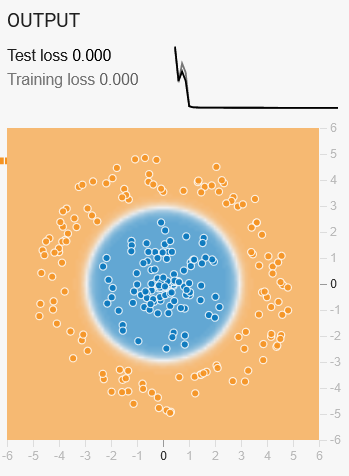
\includegraphics[width=.85\linewidth]{cs577HW1programmingQ1Data1}
    \end{subfigure}
    \begin{subfigure}{.24\textwidth}
        \centering
        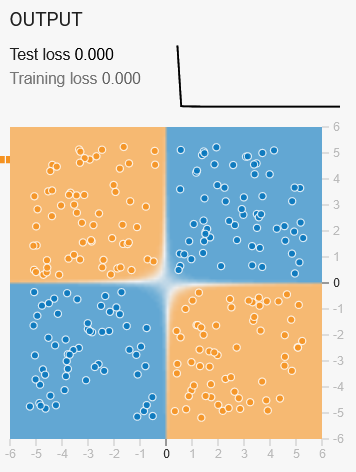
\includegraphics[width=.85\linewidth]{cs577HW1programmingQ1Data2}
    \end{subfigure}
    \begin{subfigure}{.24\textwidth}
        \centering
        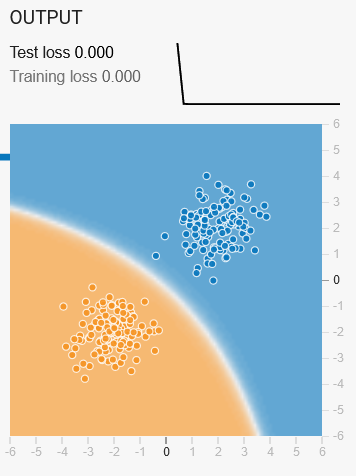
\includegraphics[width=.85\linewidth]{cs577HW1programmingQ1Data3}
    \end{subfigure}
    \begin{subfigure}{.24\textwidth}
        \centering
        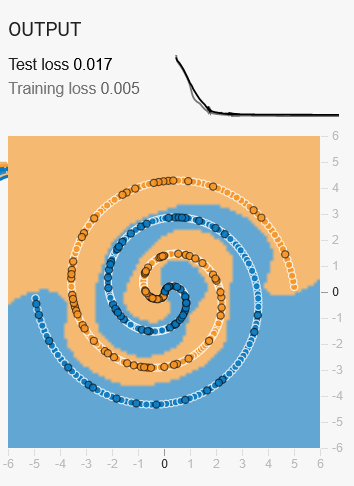
\includegraphics[width=.85\linewidth]{cs577HW1programmingQ1Data4}
    \end{subfigure}
    \caption{4 classification results in tensorflow playground}
    \label{fig:classificationPlayground}
\end{figure}

\section*{Question 2}
\subsection*{Problem statement}
image tri-class classification problem
\subsection*{Proposed solution}
as asked, use densely connected neural networks to classify the classes.
\subsection*{Implementation details}
I will use colab to do all the work. The dataset are load from tensorflow.datasets so no extra link. The classes I pick are the first three.

The training image is vectorized and converted to value between \(0\) and \(1\), and their labels are already in integers so no further process on it.
The tuning process is summarized in the following tables

\begin{center}
    \begin{tabular}{ccccc}\hline
        NN architecture & activation & optimizer & epoch & batch size \\ \hline
        (64,64,3) & (relu,relu,softmax) & rmsprop, lr=0.001 & 20 & 512\\
        (64,64,3) & (relu,relu,softmax) & rmsprop, lr=0.001 & 100 & 1024\\
        (64,64,3) & (relu,relu,softmax) & rmsprop, lr=0.001 & 200 & 1024\\
        (64,64,3) & (relu,relu,softmax) & rmsprop, lr=0.001 & 75 & 1024\\
        (64,64,3) & (Tanh,Tanh,softmax) & rmsprop, lr=0.001 & 75 & 1024\\
        (64,64,64,64,3) & (relu,...,relu,softmax) & rmsprop, lr=0.001 & 75 & 1024\\
        (99,99,99,99,3) & (relu,...,relu,softmax) & rmsprop, lr=0.001 & 75 & 1024\\
        ($64_{\times 7}$,3) & (relu,...,relu,softmax) & rmsprop, lr=0.001 & 75 & 1024\\
        \hline
    \end{tabular}
\end{center}
\begin{center}
    \begin{tabular}{ccccc}\hline
        loss & acc & val loss & val acc & comment on next tuning\\ \hline
        0.7066 & 0.7066 & 0.6712 & 0.7153 & haven't cvg yet and need bigger batch size\\
        0.5245 & 0.7851 & 0.5729 & 0.7767 & haven't cvg yet, but batch size enough\\
        0.3873 & 0.8447 & 0.5927 & 0.7787 & actually overfit after 75 epoch\\
        0.5873 & 0.7577 & 0.5944 & 0.7547 & tune activation\\
        0.5590 & 0.7662 & 0.6739 & 0.7167 & not good, tune NN\\
        0.5394 & 0.7780 & 0.5991 & 0.7620 & better, try more units then\\
        0.5830 & 0.7582 & 0.6156 & 0.7413 & not good, try more layers then\\
        0.5597 & 0.7648 & 0.6177 & 0.7467 & no big improvement, so save the 6th model\\
        \hline
    \end{tabular}
\end{center}

The loss vs epoch and accuracy vs epoch figures are below; row 1 and row 3 are loss vs epoch and row 2 and row 4 are accuracy vs epoch.

\begin{figure}[h!]
    \centering
    \begin{subfigure}{.24\textwidth}
        \centering
        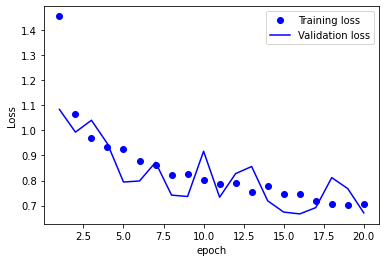
\includegraphics[width=.85\linewidth]{cs577HW1programmingQ2Try1LosEpoch}
    \end{subfigure}
    \begin{subfigure}{.24\textwidth}
        \centering
        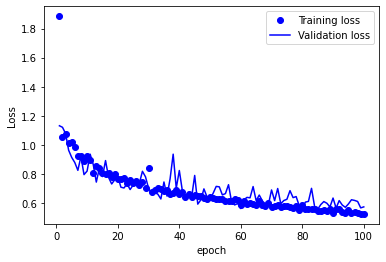
\includegraphics[width=.85\linewidth]{cs577HW1programmingQ2Try2LosEpoch}
    \end{subfigure}
    \begin{subfigure}{.24\textwidth}
        \centering
        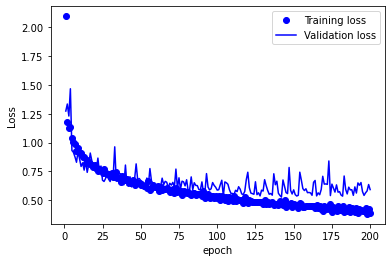
\includegraphics[width=.85\linewidth]{cs577HW1programmingQ2Try3LosEpoch}
    \end{subfigure}
    \begin{subfigure}{.24\textwidth}
        \centering
        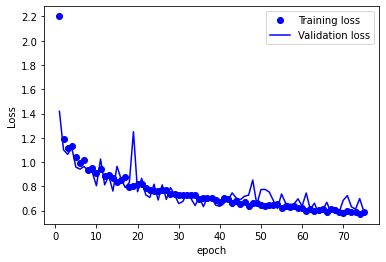
\includegraphics[width=.85\linewidth]{cs577HW1programmingQ2Try4LosEpoch}
    \end{subfigure}\\
    \begin{subfigure}{.24\textwidth}
        \centering
        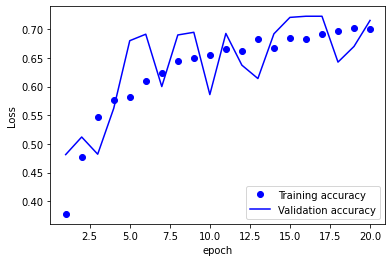
\includegraphics[width=.85\linewidth]{cs577HW1programmingQ2Try1AccEpoch}
    \end{subfigure}
    \begin{subfigure}{.24\textwidth}
        \centering
        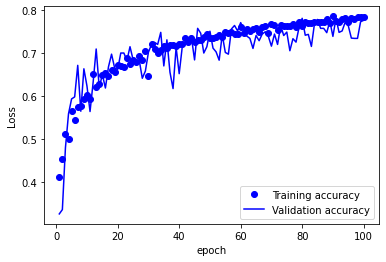
\includegraphics[width=.85\linewidth]{cs577HW1programmingQ2Try2AccEpoch}
    \end{subfigure}
    \begin{subfigure}{.24\textwidth}
        \centering
        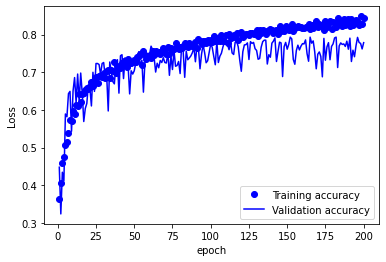
\includegraphics[width=.85\linewidth]{cs577HW1programmingQ2Try3AccEpoch}
    \end{subfigure}
    \begin{subfigure}{.24\textwidth}
        \centering
        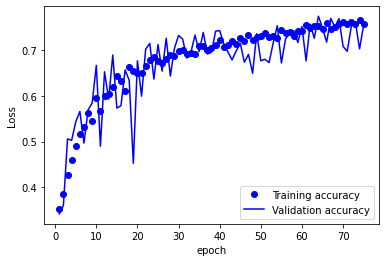
\includegraphics[width=.85\linewidth]{cs577HW1programmingQ2Try4AccEpoch}
    \end{subfigure}\\
    \begin{subfigure}{.24\textwidth}
        \centering
        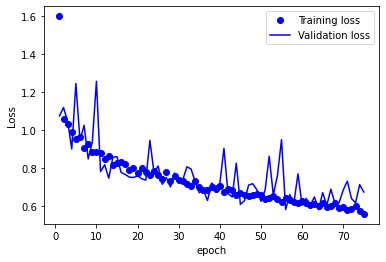
\includegraphics[width=.85\linewidth]{cs577HW1programmingQ2Try5LosEpoch}
    \end{subfigure}
    \begin{subfigure}{.24\textwidth}
        \centering
        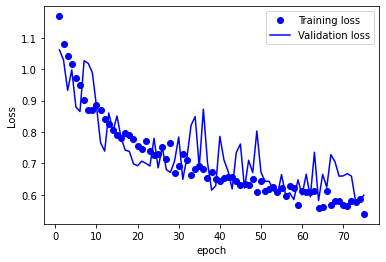
\includegraphics[width=.85\linewidth]{cs577HW1programmingQ2Try6LosEpoch}
    \end{subfigure}
    \begin{subfigure}{.24\textwidth}
        \centering
        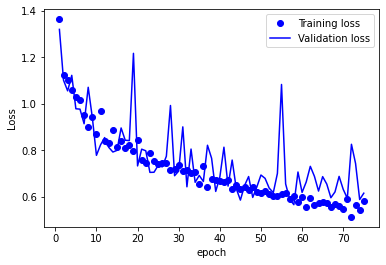
\includegraphics[width=.85\linewidth]{cs577HW1programmingQ2Try7LosEpoch}
    \end{subfigure}
    \begin{subfigure}{.24\textwidth}
        \centering
        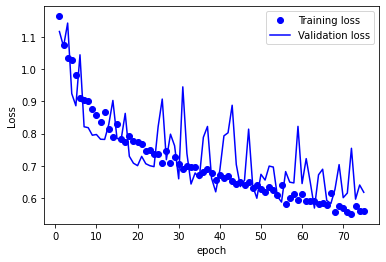
\includegraphics[width=.85\linewidth]{cs577HW1programmingQ2Try8LosEpoch}
    \end{subfigure}\\
    \begin{subfigure}{.24\textwidth}
        \centering
        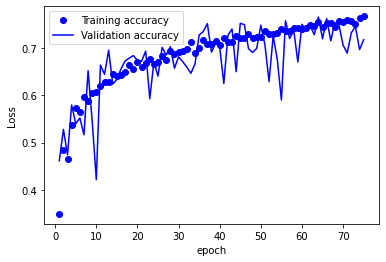
\includegraphics[width=.85\linewidth]{cs577HW1programmingQ2Try5AccEpoch}
    \end{subfigure}
    \begin{subfigure}{.24\textwidth}
        \centering
        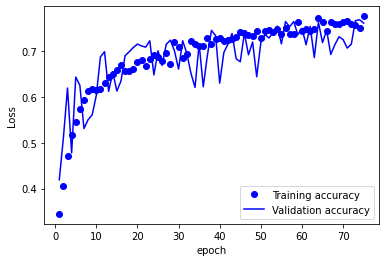
\includegraphics[width=.85\linewidth]{cs577HW1programmingQ2Try6AccEpoch}
    \end{subfigure}
    \begin{subfigure}{.24\textwidth}
        \centering
        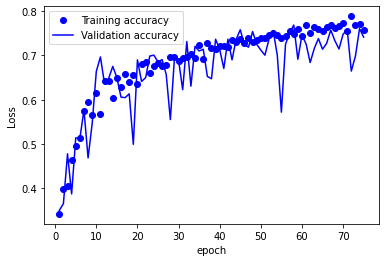
\includegraphics[width=.85\linewidth]{cs577HW1programmingQ2Try7AccEpoch}
    \end{subfigure}
    \begin{subfigure}{.24\textwidth}
        \centering
        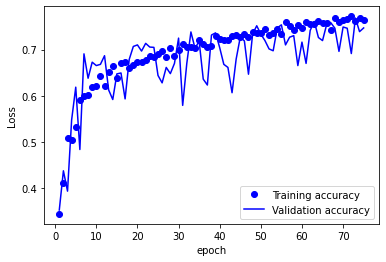
\includegraphics[width=.85\linewidth]{cs577HW1programmingQ2Try8AccEpoch}
    \end{subfigure}
    \caption{subset cifar 10 classification tuning checkpoints}
    \label{fig:cifar10triClass}
\end{figure}


\subsection*{Results and discussion}

\begin{itemize}
    \item train data size: 15000-1500
    \item validation data size: 1500
    \item test data size: 3000
    \item test acc: 0.7436
\end{itemize}

I know there'll could be better result, but considering the limited time, I am satisfied for the result.

The saved model is uploaded to a github repo, and the link is contained in both the notebook file and models.txt.


\section*{Question 3}

\subsection*{Problem statement}
text bi-class classification problem, non-spam or spam.
\subsection*{Proposed solution}
same as last one
\subsection*{Implementation details}
same as last one and here're the result tables and figures


\begin{center}
    \begin{tabular}{ccccc}\hline
        NN architecture & activation & optimizer & epoch & batch size \\ \hline
        (64,64,3) & (relu,relu,softmax) & rmsprop, lr=0.001 & 20 & 512\\
        (64,64,3) & (relu,relu,softmax) & rmsprop, lr=0.0005 & 100 & 512\\
        (64,64,3) & (relu,relu,softmax) & rmsprop, lr=0.0005 & 30 & 512\\
        \hline
    \end{tabular}
\end{center}
\begin{center}
    \begin{tabular}{ccccc}\hline
        loss & acc & val loss & val acc & comment on next tuning\\ \hline
        0.1602 & 0.9390 & 0.1911 & 0.9325 & not cvg and cvg too fast; need smaller lr, more epoch to see if overfit\\
        0.0849 & 0.9734 & 0.1581 & 0.9425 & better, now maybe stop at 30 epoch\\
        0.1725 & 0.9379 & 0.2057 & 0.9300 & i could stop here \\
        \hline
    \end{tabular}
\end{center}

The loss vs epoch and accuracy vs epoch figures are below; row 1 are loss vs epoch and row 2 are accuracy vs epoch.

\begin{figure}[h!]
    \centering
    \begin{subfigure}{.32\textwidth}
        \centering
        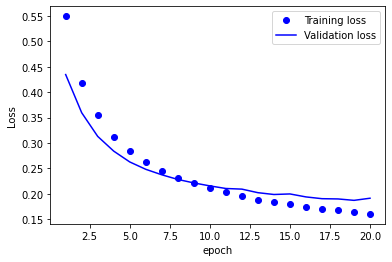
\includegraphics[width=.85\linewidth]{cs577HW1programmingQ3Try1LosEpoch}
    \end{subfigure}
    \begin{subfigure}{.32\textwidth}
        \centering
        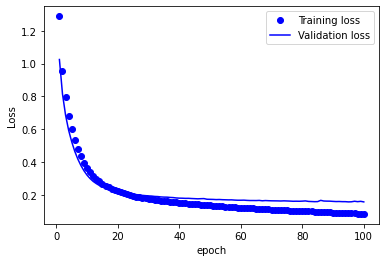
\includegraphics[width=.85\linewidth]{cs577HW1programmingQ3Try2LosEpoch}
    \end{subfigure}
    \begin{subfigure}{.32\textwidth}
        \centering
        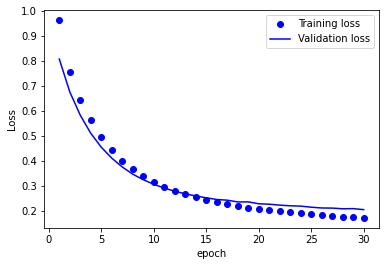
\includegraphics[width=.85\linewidth]{cs577HW1programmingQ3Try3LosEpoch}
    \end{subfigure}\\
    \begin{subfigure}{.32\textwidth}
        \centering
        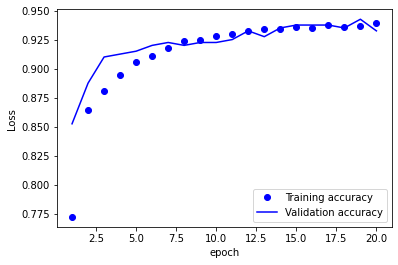
\includegraphics[width=.85\linewidth]{cs577HW1programmingQ3Try1AccEpoch}
    \end{subfigure}
    \begin{subfigure}{.32\textwidth}
        \centering
        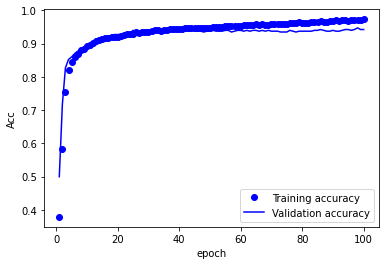
\includegraphics[width=.85\linewidth]{cs577HW1programmingQ3Try2AccEpoch}
    \end{subfigure}
    \begin{subfigure}{.32\textwidth}
        \centering
        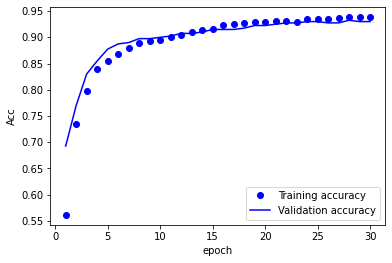
\includegraphics[width=.85\linewidth]{cs577HW1programmingQ3Try3AccEpoch}
    \end{subfigure}
    \caption{spambase data bi-class classification tuning checkpoints}
    \label{fig:spambaseBiClass}
\end{figure}


\subsection*{Results and discussion}

\begin{itemize}
    \item train data size: 3220-400
    \item validation data size: 400
    \item test data size: 1381
    \item test acc: 0.9399
\end{itemize}

I'm pretty amazed on how easy this task is. Though clearly there could be a better result, but I am satisfied enough to carry on to the last question.



\section*{Question 4}

\subsection*{Problem statement}

a regression problem,

\subsection*{Proposed solution}

as asked, use densely connected neural networks to do regression task.

\subsection*{Implementation details}

About the dataset, it contains various missing values, spreading all the place, and no full rows. In this case, I will discard several columns of data for whose missing value percentage is about 60 percent or higher.

In all, the discarded columns represents
\begin{itemize}
    \item LemasSwornFT: number of sworn full time police officers
    \item LemasSwFTPerPop: sworn full time police officers per 100K population
    \item LemasSwFTFieldOps: number of sworn full time police officers in field operations
    \item LemasSwFTFieldPerPop: sworn full time police officers in field operations
    \item LemasTotalReq: total requests for police
    \item LemasTotReqPerPop: total requests for police per 100K popuation
    \item PolicReqPerOffic: total requests for police per police officer
    \item PolicPerPop: police officers per 100K population
    \item RacialMatchCommPol: a measure of the racial match between the community and the police force. High values indicate proportions in community and police force are similar
    \item PctPolicWhite: percent of police that are caucasian
    \item PctPolicBlack: percent of police that are african american
    \item PctPolicHisp: percent of police that are hispanic
    \item PctPolicAsian: percent of police that are asian
    \item PctPolicMinor: percent of police that are minority of any kind
    \item OfficAssgnDrugUnits: number of officers assigned to special drug units
    \item NumKindsDrugsSeiz: number of different kinds of drugs seized
    \item PolicAveOTWorked: police average overtime worked
    \item PolicCars: number of police cars 
    \item PolicOperBudg: police operating budget
    \item LemasPctPolicOnPatr: percent of sworn full time police officers on patrol
    \item LemasGangUnitDeploy: gang unit deployed
    \item PolicBudgPerPop: police operating budget per population
\end{itemize}

Next found that the first 5 column of data are non-predictive, I will also discard them.

Last step, delete rows containing the rest missing values, and transform the strings form to numerical form.

Then after normalizing using training dataset, we start to train the NN. Here's the table for tuning results. Note across them the following hyperparameters are maintained

\begin{itemize}
    \item NN architecture: (64,64,3) 
    \item activation: (relu,relu,softmax) 
    \item optimizer: rmsprop, lr=0.001
\end{itemize}


\begin{center}
    \begin{tabular}{cccc}\hline
        epoch& batch size & mean validate mae & comment on next tune\\ \hline
        20 & 1 & 0.1083 & not cvg yet, need more epoch to see if overfit\\
        100 & 1 & 0.1107 & still\\
        200 & 1 & 0.1163 & I could stop here\\
        \hline
    \end{tabular}
\end{center}

The loss vs epoch and accuracy vs epoch figures are below; row 1 are loss vs epoch and row 2 are accuracy vs epoch.

\begin{figure}[h!]
    \centering
    \begin{subfigure}{.32\textwidth}
        \centering
        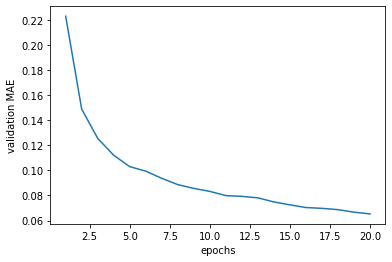
\includegraphics[width=.85\linewidth]{cs577HW1programmingQ4Try1ValMAEEpoch}
    \end{subfigure}
    \begin{subfigure}{.32\textwidth}
        \centering
        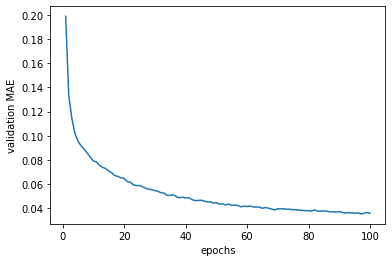
\includegraphics[width=.85\linewidth]{cs577HW1programmingQ4Try2ValMAEEpoch}
    \end{subfigure}
    \begin{subfigure}{.32\textwidth}
        \centering
        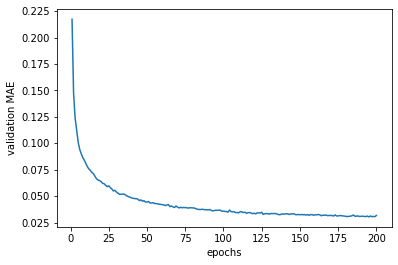
\includegraphics[width=.85\linewidth]{cs577HW1programmingQ4Try3ValMAEEpoch}
    \end{subfigure}
    \caption{crime Rate regression tuning checkpoints}
    \label{fig:crimeRegre}
\end{figure}


\subsection*{Results and discussion}

\begin{itemize}
    \item train data size: 1047
    \item validation data size: 348
    \item test data size: 598
    \item test acc: 0.09977
\end{itemize}

More smooth than I expected.


\newpage

%\bibliographystyle{acm}
%\bibliography{D:/Papers.bib}

\newpage
\appendix
%\section{Appendix}

\end{document}